\chapter{Firmware Development and Experimental Validation}
\label{chap:firmware}

\section{Development Environment: ESP32 and PlatformIO}

The OMNICAR project utilizes the ESP32 microcontroller as the core low-level control unit. Given the necessity to manage high-frequency tasks—such as reading four independent encoders and executing real-time control loops—the development environment played a critical role in ensuring system reliability. While the Arduino IDE is suitable for rapid prototyping, it lacks the advanced features required for complex, multi-file robotic projects. Consequently, the development was migrated to \textbf{PlatformIO}, an open-source ecosystem for IoT development integrated into Visual Studio Code.

The choice of PlatformIO was driven by several technical advantages essential for the OMNICAR's firmware architecture:

\begin{itemize}
    \item \textbf{Modular Project Structure}: Unlike the flat file structure of Arduino, PlatformIO encourages a professional C++ organization. By separating declarations in header files (\texttt{.h}) and logic in implementation files (\texttt{.cpp}), the project achieved better encapsulation and significantly reduced compilation times through incremental builds.
    \item \textbf{Advanced Debugging and Monitoring}: The integrated serial monitor, configured at 115200 baud, allowed for real-time telemetry of motor speeds and PID performance. Furthermore, the environment's support for hardware debugging was pivotal during the initial validation of the encoder reading tasks.
    \item \textbf{Remote Deployment and Diagnostics (OTA)}: Since the OMNICAR is a mobile platform, frequent firmware updates via USB were impractical during dynamic field tests. PlatformIO's native support for \textbf{ArduinoOTA} (Over-The-Air) enabled wireless flashing of the ESP32 over the local network, allowing for immediate iterations. Furthermore, this setup facilitated the analysis of offline floor tests by sharing log files through an integrated \textbf{Web Server} hosted on the ESP32's IP address, eliminating the need for physical access to the robot's internal hardware.
\end{itemize}

\subsection{Configuration: the platformio.ini file}

The \texttt{platformio.ini} file is the core of the project configuration. It allows for precise control over the compilation environment, library versions, and upload methods. Below is the specific setup used for the OMNICAR:

\begin{vscode}{platformio.ini}
[env:esp32dev]
platform = espressif32 @ 6.5.0
board = esp32dev
framework = arduino

; Over-the-Air update configuration
upload_protocol = espota
upload_port = 192.168.31.144  	; IP address ESP32

monitor_speed = 115200 		  	;BaudRate serial monitor
lib_deps = 
    adafruit/Adafruit ADS1X15 @ ^2.5.0
    adafruit/Adafruit BusIO @ ^1.14.1
    bblanchon/ArduinoJson @ ^6.21.3

build_flags = 
    -D CORE_DEBUG_LEVEL=3
    -D _USE_MATH_DEFINES

build_src_filter = +<*> -<PID.cpp>
\end{vscode}

As previously mentioned, the implementation of the \texttt{espota} protocol proved to be fundamental during the experimental phase. It enabled wireless firmware updates while the robot remained positioned on the floor, thereby eliminating the need for constant physical tethering.

\section{Software Architecture and Project Structure}

The firmware is developed using an Object-Oriented Programming (OOP) approach to manage the complexity of the four-wheeled omnidirectional system. The separation of declarations (\texttt{.h}) and implementations (\texttt{.cpp}) is fundamental to ensure modularity (module like motor, encoder, communication, control), allowing for independent testing of hardware components like motors and encoders.

The ESP32 project hierarchy, as organized within the PlatformIO environment, is structured as follows:

\begin{folderbox}{ESP32 Project Directory Structure}
\dirtree{%
.1 OmniCar\_Control/[02]Code/Omnicar/.
.2 .pio/ \DTcomment{Build files and libraries}.
.2 include/ \DTcomment{Header files (.h)}.
.3 connection.h \DTcomment{WiFi and MQTT protocols}.
.3 log.h \DTcomment{Serial and network log}.
.3 motor.h \DTcomment{Control interface (PWM/DIR)}.
.3 CtrlPID.h \DTcomment{PID control class}.
.3 robot.h \DTcomment{Robot class aggregation}.
.3 robot\_config.h \DTcomment{Hardware pins and kinematics}.
.3 encoder.h \DTcomment{Encoder and speed estimation}.
.2 lib/ \DTcomment{External managed libraries}.
.3 Adafruit\_ADS1115.
.3 Adafruit\_BusIO.
.3 ArduinoJson.
.2 src/ \DTcomment{Implementation files (.cpp)}.
.3 main.cpp \DTcomment{Core logic and loops}.
.3 connection.cpp.
.3 motor.cpp.
.3 CtrlPID.cpp.
.3 robot.cpp.
.3 encoder.cpp.
.2 platformio.ini \DTcomment{Build configuration}.
}
\end{folderbox}

\subsection{Role of Main Components}
To ensure a clear distinction between high-level logic and low-level hardware control, the following roles have been assigned to the primary modules:

\begin{itemize}
    \item \textbf{Robot Class (\texttt{Robot.h/cpp})}: 
    Acts as the central hardware abstraction layer and orchestrator for the firmware. It encapsulates the state of the entire platform by aggregating instances of \texttt{Motor} objects and PID controllers. It is responsible for executing the main control loop at a deterministic frequency (e.g., 50Hz, 100Hz, 200Hz), updating the kinematic model, and synchronizing the flow of data between the low-level hardware (actuators/sensors) and the communication layer.

    \item \textbf{Motor \& Encoders}: 
    These low-level modules handle the direct interface with the hardware drivers. The Motor module translates velocity setpoints into PWM signals (using ESP32 peripherals or external drivers like MDD10A) to control the motors. The Encoder module processes signals—capturing ticks via interrupts or dedicated hardware—to compute real-time angular position and velocity for the feedback loop.

    \item \textbf{Connection Handler}: 
    Manages the communication bridge between the embedded controller (ESP32) and the high-level planner (Raspberry Pi/ROS). It implements the protocol stack to parse incoming command packets (e.g., velocity vectors) and serializes telemetry data (encoders, battery status). It supports multiple transport layers, such as high-speed Serial (UART) for real-time control or MQTT/WiFi for remote monitoring and logging.

    \item \textbf{Robot Config (\texttt{robot\_config.h})}: 
    A centralized configuration header that serves as the "single source of truth" for the system. It contains all calibrated hardware constants—such as pin mappings, kinematic dimensions, gear ratios, and PID gains. This decoupling prevents hard-coded values in the logic files, facilitating easy tuning and adaptation to different hardware revisions without modifying the core source code.
    
\end{itemize}

\section{Hardware Abstraction: robot\_config.h}

The \texttt{robot\_config.h} file acts as a centralized configuration hub. It contains critical hardware parameters such as:
\begin{itemize}
    \item \textbf{Pin Mapping}: GPIO assignments for PWM and DIR signals for the four MDD10A drivers.
    \item \textbf{Kinematics}: Wheel radius, gear ratios, and robot geometry ($L$ and $l$ distances).
    \item \textbf{Encoder Resolution}: Definition of the counts per revolution (CPR) to ensure accurate odometry.
\end{itemize}

The \texttt{robot\_config.h} file acts as a centralized configuration hub, ensuring decoupling between hardware parameters and control logic. It contains critical system constants such as:
\begin{itemize}
    \item \textbf{Pin Mapping}: GPIO assignments for the PWM and DIR (direction) peripherals and digital inputs for the encoder signals.
    \item \textbf{Kinematics}: Geometric definitions for the omnidirectional model, including wheel radius ($r = 0.06$ m), gear ratio ($N = 18.75$), and chassis half-dimensions ($L_x = 0.185$ m, $L_y = 0.220$ m).
    \item \textbf{Encoder Resolution}: Definition of the counts per revolution ($CPR = 64$) used to convert raw ticks into angular velocity.
    \item \textbf{PID Control Tuning}: Specifies the PI controller gains derived via \textit{Internal Model Control} (IMC). The parameters are calculated based on an identified first-order plant model of the motors 
\end{itemize}


\section{Experimental Procedures and Main Loop}

The firmware's operational core is encapsulated within the \texttt{main.cpp} file, which manages the real-time execution loop for the motion control algorithms.

\subsection{System Initialization and Setup}
The \texttt{setup()} function defines a common initialization phase for all experimental procedures. This routine configures the hardware peripherals and communication protocols required for robot operation. Include the initialization of the serial interface at 115,200 baud for telemetry, the configuration of the \texttt{Robot} object, and the setup of the Over-The-Air (OTA) update system.

The \texttt{robot.init()} method assigns the GPIO pins for the MDD10A motor drivers and read the encoder channels. A serial channel protocol is initialized to exchange data between the ESP32 and the Raspberry Pi 5.

\begin{vscode}{main.cpp/setup}
void setup() {
  // Inizializza la seriale per il monitoraggio
  Serial.begin(115200);
  serial_channels.init(processSerialPacket, serialWrite);
  // Configura il pulsante BOOT (GPIO 0)
  pinMode(0, INPUT_PULLUP);

  // --- WIFI, OTA, WEB SERVER SETUP ---
  setupWiFi();
  setupOTA();
  // setupWebServer(); //Web Server usato per scaricare i file di log durante le prove offline

  Serial.println("--- OMNICAR MOTOR TEST START ---");
  Serial.flush();
  // Inizializza il robot passando la funzione di callback per la seriale
  robot.init(serialWriteChannel);
  Serial.println("Robot initialized.");
  
  // Reset signal
  serialWriteChannel('r', 0);
  // Initialization
  current_micros = micros();
  previous_micros = current_micros;
  last_motor_update_millis = millis();
}
\end{vscode}

\subsection{Encoder Validation and Tick Counting}
The initial experimental phase consisted of a manual rotation test performed on a selected motor to calibrate and validate the encoder resolution. Although the hardware specifications indicated a nominal resolution of 1200 pulses per revolution (ppr), this empirical verification was essential to ensure that the software parameters defined in \texttt{robot\_config.h} accurately reflected the physical behavior of the system. This procedure eliminated potential discrepancies between the theoretical datasheet and the real-time pulse counting logic, providing a reliable foundation for the first-order velocity control loop.

\begin{vscode}{main.cpp/loop\_manuale}
void loop() {
  uint32_t dt = 0; // Variabile delta time per robot.update
  int idx_mot = 0;
  Serial.println("   TEST MANUALE ENCODER (Ruota a mano)/\n Inserisci indice motore (0-3) per iniziare.");

  while (Serial.available() == 0) {
    delay(10);
  }

  idx_mot = Serial.parseInt();
  // Pulisci il buffer seriale (rimuovi newline)
  while (Serial.available()) { Serial.read(); }

  if (idx_mot >= 0 && idx_mot < kNumMot) {
    Serial.printf("--> MONITORAGGIO MOTORE %d ATTIVO\n", idx_mot);
    Serial.println("    Ruota la ruota manualmente.");

    robot.setMotorPWM(idx_mot, 0);

    // Loop finché non si riceve input seriale
    while (Serial.available() == 0) {
      robot.update(dt);
      Serial.printf("MOT[%d] | Ticks: %d | Odo: %d\n", idx_mot, robot.enc[idx_mot].tick, robot.enc[idx_mot].odo);
    }
  } else {
    Serial.printf("Indice %d non valido! Inserire 0, 1, 2 o 3.\n", idx_mot);
  }
}
\end{vscode}

\subsection{Open-Loop Response and First-Order Approximation}
Individual motors were driven at specific PWM duty cycles to validate the assumption of a \textbf{first-order system} model. To derive this model, we consider the electromechanical equations of a DC motor in the Laplace domain ($s$-domain):

\begin{equation}
\begin{cases}
    U(s) = (R + sL)I(s) + K\Omega(s) \\
    sJ\Omega(s) = KI(s) - B\Omega(s) - T_q
\end{cases}
\begin{cases}
    U(s) = (R + sL)I(s) + K\Omega(s) \\
    KI(s) = (sJ + B)\Omega(s) + T_q
\end{cases}
\end{equation}

where $U(s)$ is the input voltage, $I(s)$ the armature current, $\Omega(s)$ the angular velocity, and $T_q$ represents the load torque. 

\subsubsection{Linearization and Order Reduction}
It is important to note that a linear transfer function $\frac{\Omega(s)}{U(s)}$ cannot be directly deduced from the equations above because the term $T_q$ renders the expression affine rather than linear. To achieve a linear representation, we assume $T_q = 0$, with the intention of compensating for this physical nonlinearity later. Under this assumption, the system can be rearranged as:

\begin{equation}
    \frac{\Omega(s)}{U(s)} = \frac{K}{(R + sL)(sJ + B)}
\end{equation}

resulting in a second-order system. In this scenario, the electrical pole ($s = -R/L$) is typically much faster (located much further left in the complex plane) than the mechanical pole ($s = -B/J$). Consequently, the high-frequency electrical dynamics can be neglected, leading to the final first-order approximation:

\begin{equation}
    G(s) = \frac{\Omega(s)}{U(s)} \approx \frac{K_{gain}}{sJ + B} = \frac{A}{\tau s + 1}
\end{equation}


\subsection{Double Step Test for PID Tuning}
As specified in the \texttt{robot\_config.h} file, the nominal control frequency was established at 50 Hz, although the system performance at higher frequencies was also evaluated in specific test cases. Prior to the formal identification of the system parameters, a preliminary test was conducted on a single motor under no-load conditions. The resulting angular velocity $\omega(t)$, measured in rad/s, is illustrated in Figure \ref{fig:First Test PWM in 50Hz}.

The experimental procedure involved a double-step input: the first step applied a PWM duty cycle of 2047 (representing approximately half of the maximum available thrust), while the second step reached the full resolution of 4095. The steady-state angular velocities observed during these tests align closely with idealized theoretical values, peaking at approximately $60$ rad/s. 

Notably, the open-loop response under no-load conditions show marginal noise and reaches the target velocity with high precision. The purely asymptotic profile of the curve provides visual confirmation that the electrical dynamics—associated with the second pole of the system—are effectively negligible compared to the mechanical time constant. This empirical evidence further justifies the adoption of a first-order approximation for the velocity control loop.

\begin{figure}[H]
    \centering
    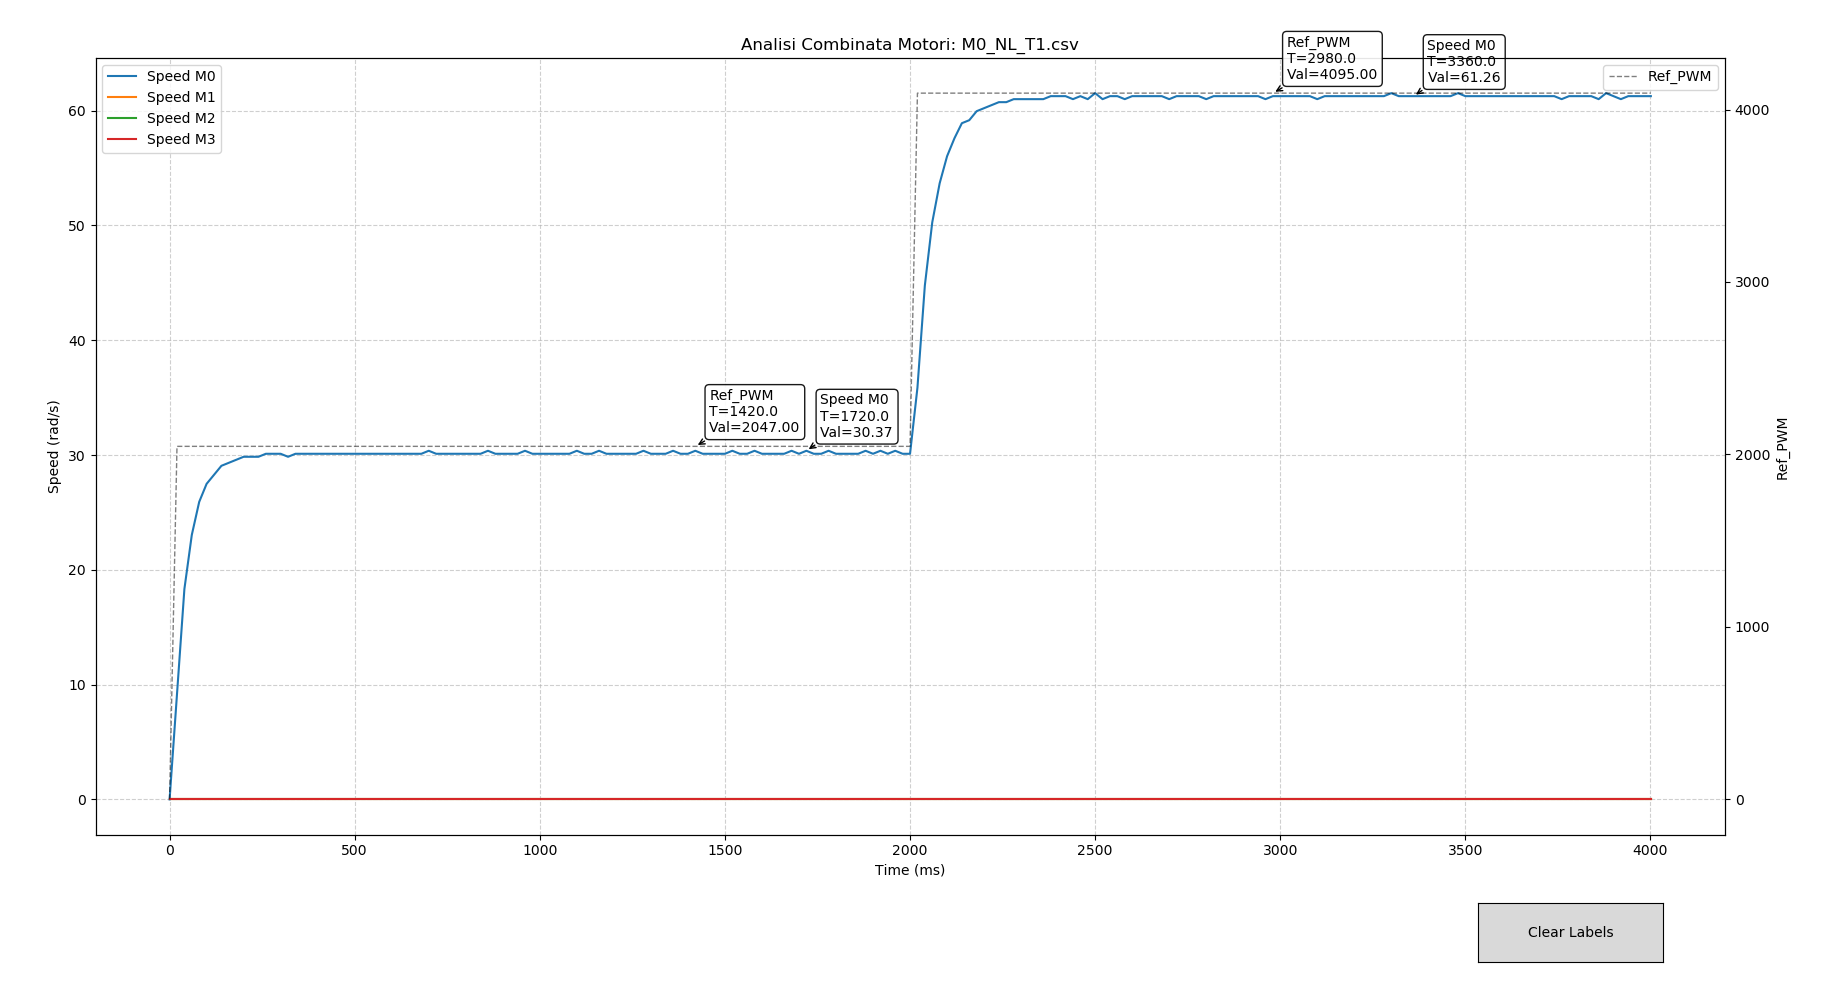
\includegraphics[width=1\textwidth]{IMG/PID/M0_Primo_TEST_PWM.png}
    \caption{First Test PWM in 50Hz}
    \label{fig:First Test PWM in 50Hz}
\end{figure}

A double-step input was applied to all four motors simultaneously during a test with load (robot on the floor). By measuring the steady-state speed we can calculating the gain and the time constant ($\tau$).

As illustrated in Figures \ref{fig:MA_NL_T2_50hz}, \ref{fig:MA_NL_T2_50hz_Mot2}, and \ref{fig:MA_NL_T2_50hz_Separato}, specific safety PWM thresholds were established for the step response tests: a first step at 750 and a second at 1500. These duty cycle values correspond approximately to angular velocities of 10 rad/s and 20 rad/s, respectively.

In this phase, isolating the individual motor responses was fundamental to detecting any potential mechanical or electrical anomalies. The experimental data confirms that all motors exhibit consistent behavior, characterized by a decoupled and uniform response across the assembly.

Based on the analysis of the collected data, the following system parameters were identified. First, the PWM signals were converted into their equivalent voltage values using the following relation:

\begin{equation}
    V_{pwm} = \frac{PWM_{ref}}{PWM_{max}} \cdot V_{battery}
\end{equation}

Given a maximum resolution $PWM_{max} = 4095$ and a measured battery voltage $V_{battery} = 11.9$ V, we obtain:

\begin{equation}
    V_{pwm,750} \approx 2.18 \text{ V}, \quad V_{pwm,1500} \approx 4.36 \text{ V}
\end{equation}

The steady-state gain $K$ was then calculated as the ratio between the variation in angular velocity and the variation in input voltage:

\begin{equation}
    K = \frac{\Delta \omega}{\Delta V_{in}} = \frac{\omega_2 - \omega_1}{V_{pwm,1500} - V_{pwm,750}} = 5.04
\end{equation}

To determine the time constant $\tau$, we identified the angular velocity value corresponding to $63.2\%$ of the transient transition between the first and second step:

\begin{equation}
    \omega_{\tau} = \omega_1 + 0.632 \cdot (\omega_2 - \omega_1) = 16.9 \text{ rad/s}
\end{equation}

By locating $\omega_{\tau}$ on the experimental temporal plot, the resulting time constant was estimated to be approximately $\tau \approx 90$ ms.

% --- Open Loop Motor Analysis (MA) Tests ---
\begin{figure}[H]
    \centering
    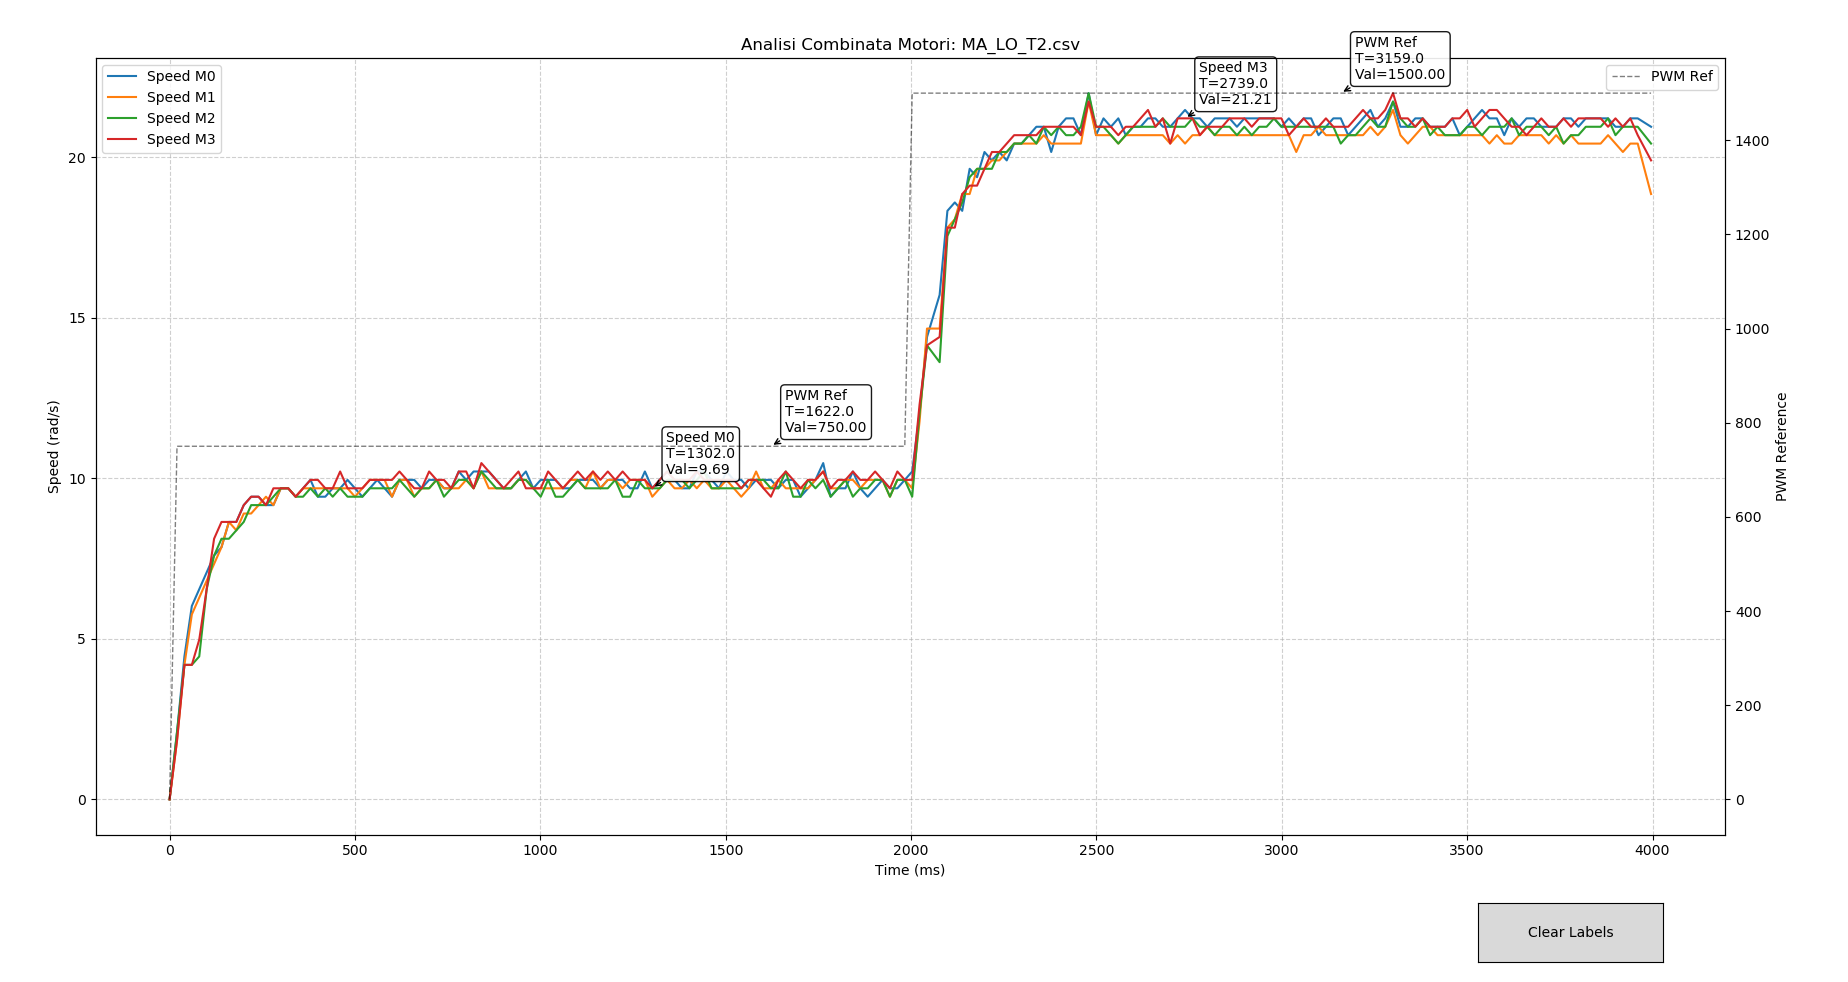
\includegraphics[width=1\textwidth]{IMG/PID/MA_NL_T2_50hz.png}
    \caption{Open-loop no-load test (MA\_NL) at a sampling frequency of 50 Hz}
    \label{fig:MA_NL_T2_50hz}
\end{figure}

\begin{figure}[H]
    \centering
    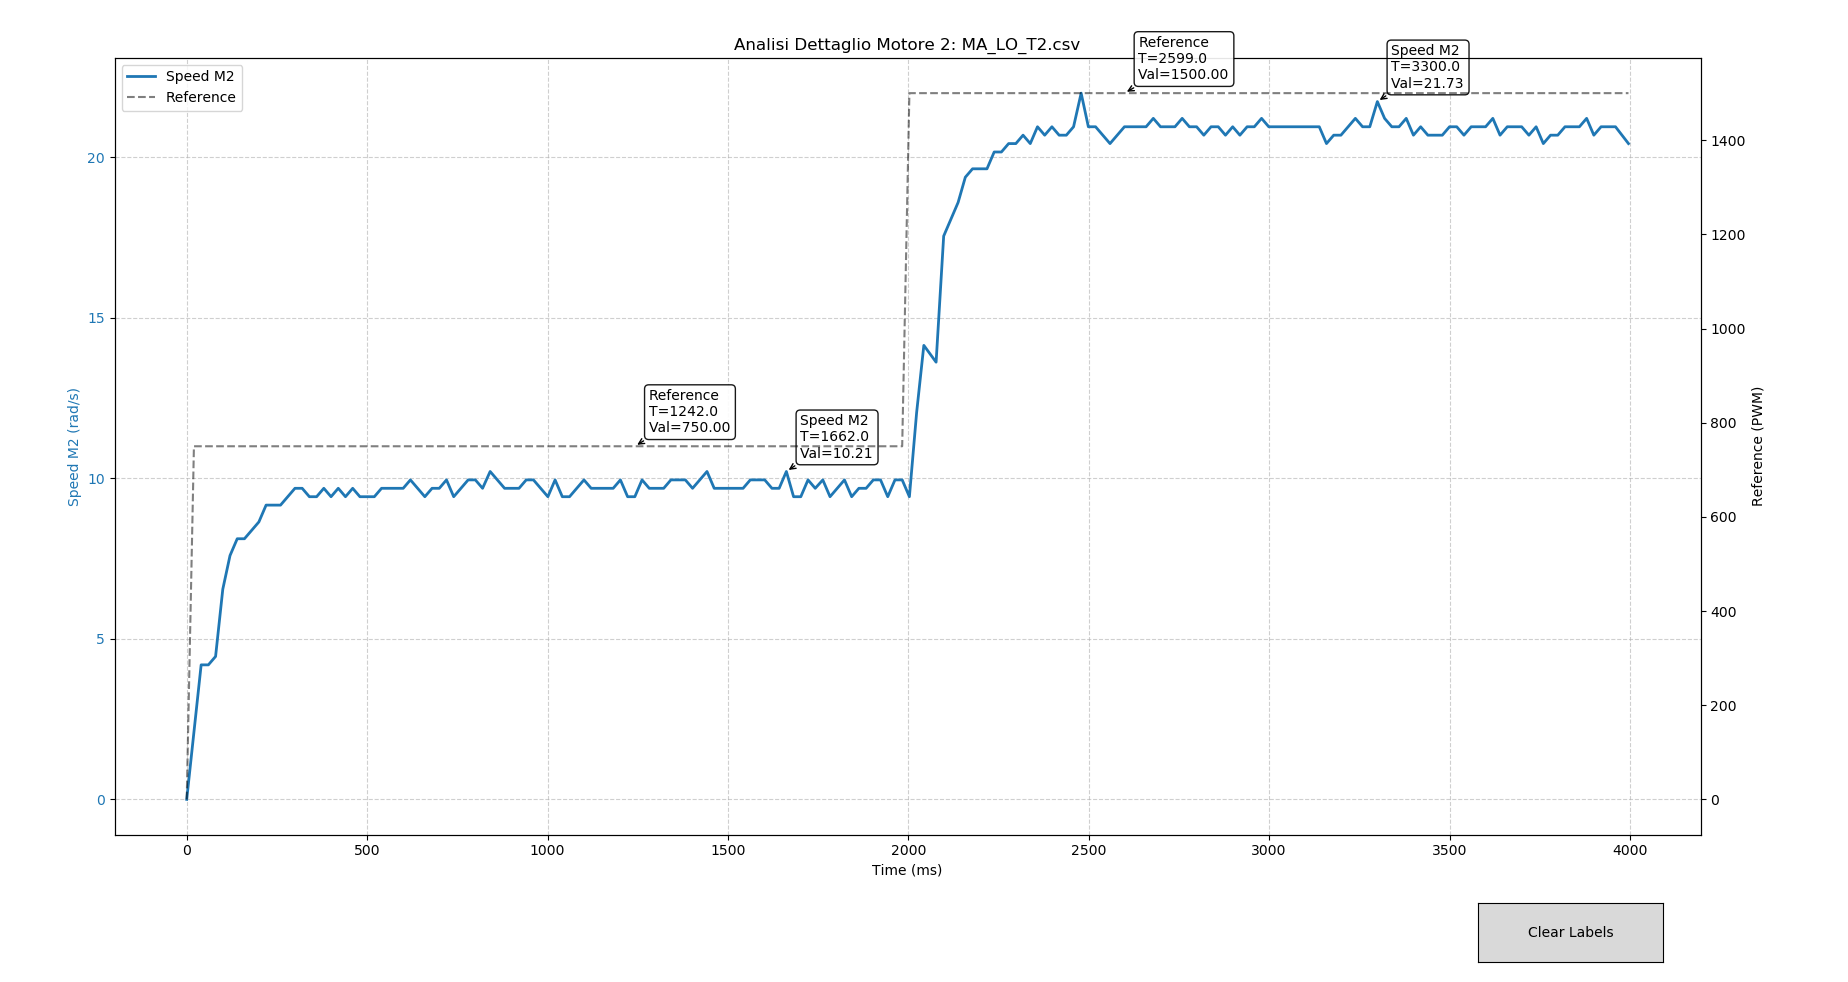
\includegraphics[width=1\textwidth]{IMG/PID/MA_NL_T2_50hz_Mot2.png}
    \caption{Open-loop velocity profile for Motor 2 at 50 Hz sampling rate}
    \label{fig:MA_NL_T2_50hz_Mot2}
\end{figure}

\begin{figure}[H]
    \centering
    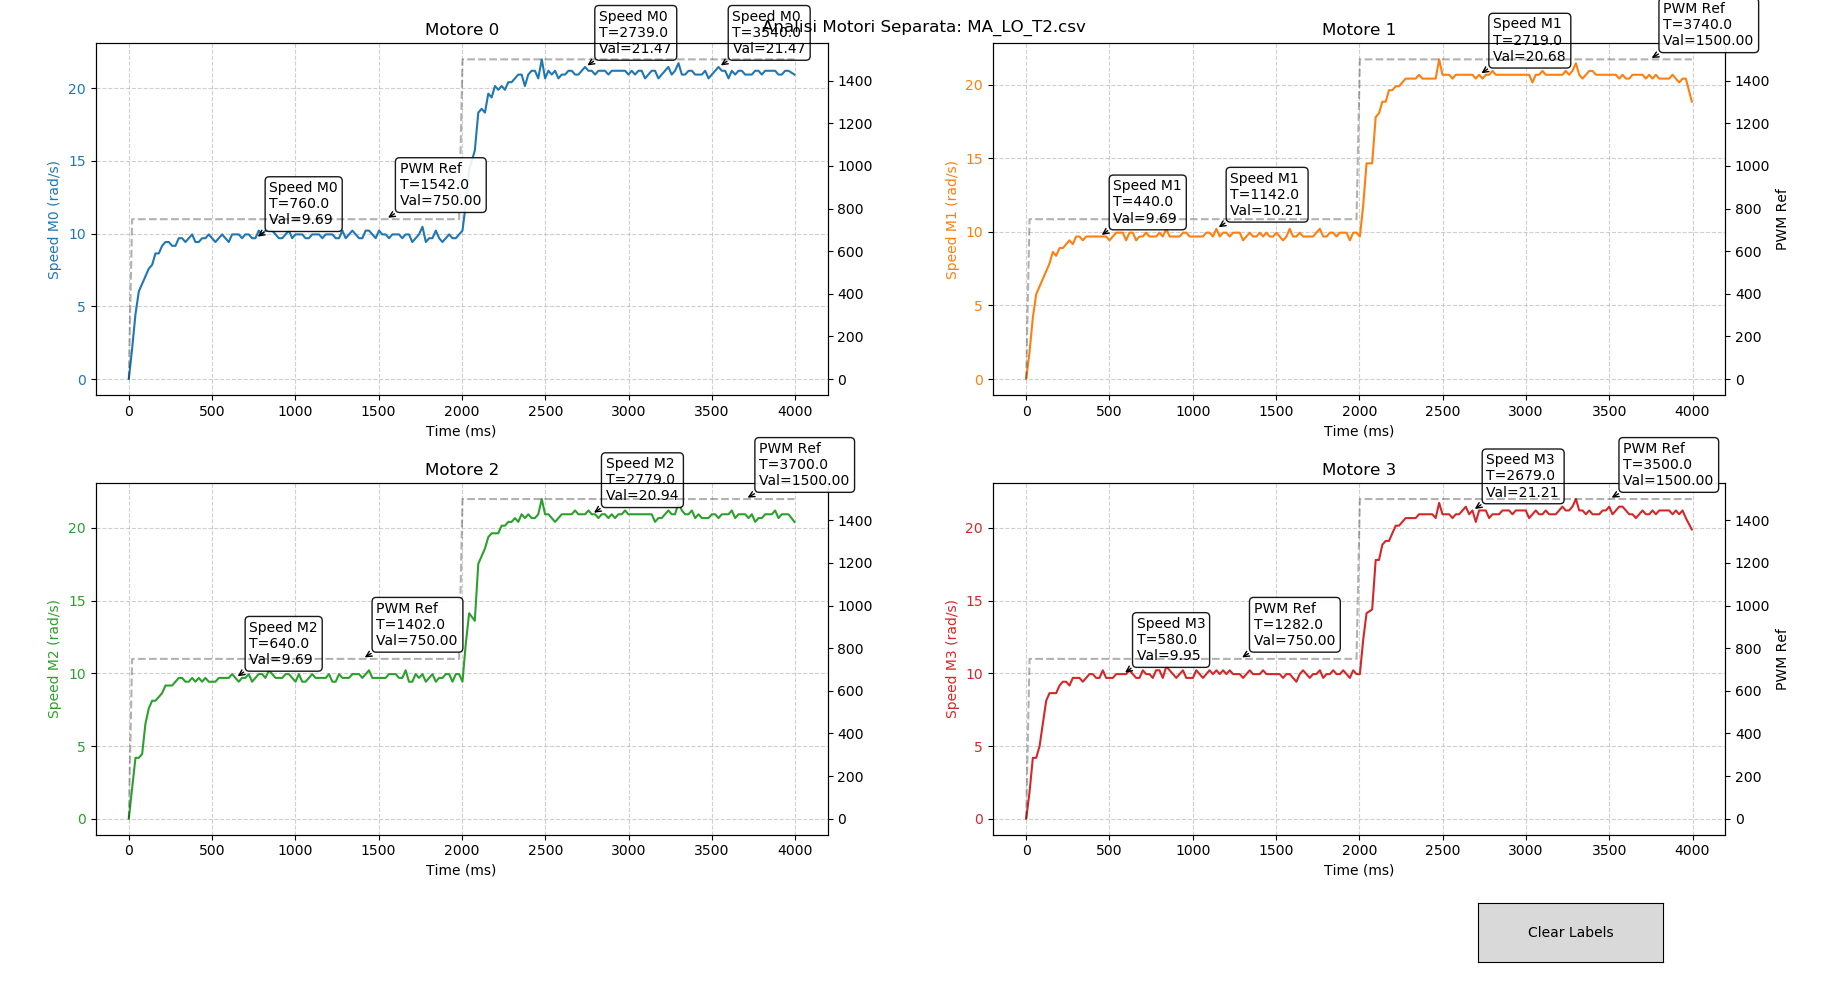
\includegraphics[width=1\textwidth]{IMG/PID/MA_NL_T2_50hz_Separato.png}
    \caption{Detailed view of the open-loop response at 50 Hz for system identification}
    \label{fig:MA_NL_T2_50hz_Separato}
\end{figure}

How show in Figure \ref{fig:MA_NL_T5_100hz}. Experimental analysis demonstrated that increasing the control frequency beyond 50 Hz significantly degrades the Signal-to-Noise Ratio (SNR) in velocity estimation. This phenomenon is primarily attributable to the reduction in numerical resolution—specifically, the quantization error of encoder ticks within shorter sampling periods—and temporal jitter affecting the \texttt{kMotCtrlTimeUs} parameter. 

At higher frequencies, interrupt management on the ESP32 introduces variable latencies that lead to asynchronous tick accumulation, resulting in periodic noise spikes. To ensure the stability of the control algorithms and prevent the amplification of these disturbances through derivative terms, the low-level control loop was maintained at 50 Hz. This configuration provides the optimal compromise between temporal determinism and signal resolution.

\par Subsequent phases of the project will involve use of a dedicated communication link with the Raspberry Pi. In this setup, the raw encoder signals will be transmitted directly and evaluated without the onboard conversion to radians. This approach is designed to assess the signal integrity and the effectiveness of processing when operating at sampling frequencies exceeding 50 Hz.

\begin{figure}[H]
    \centering
    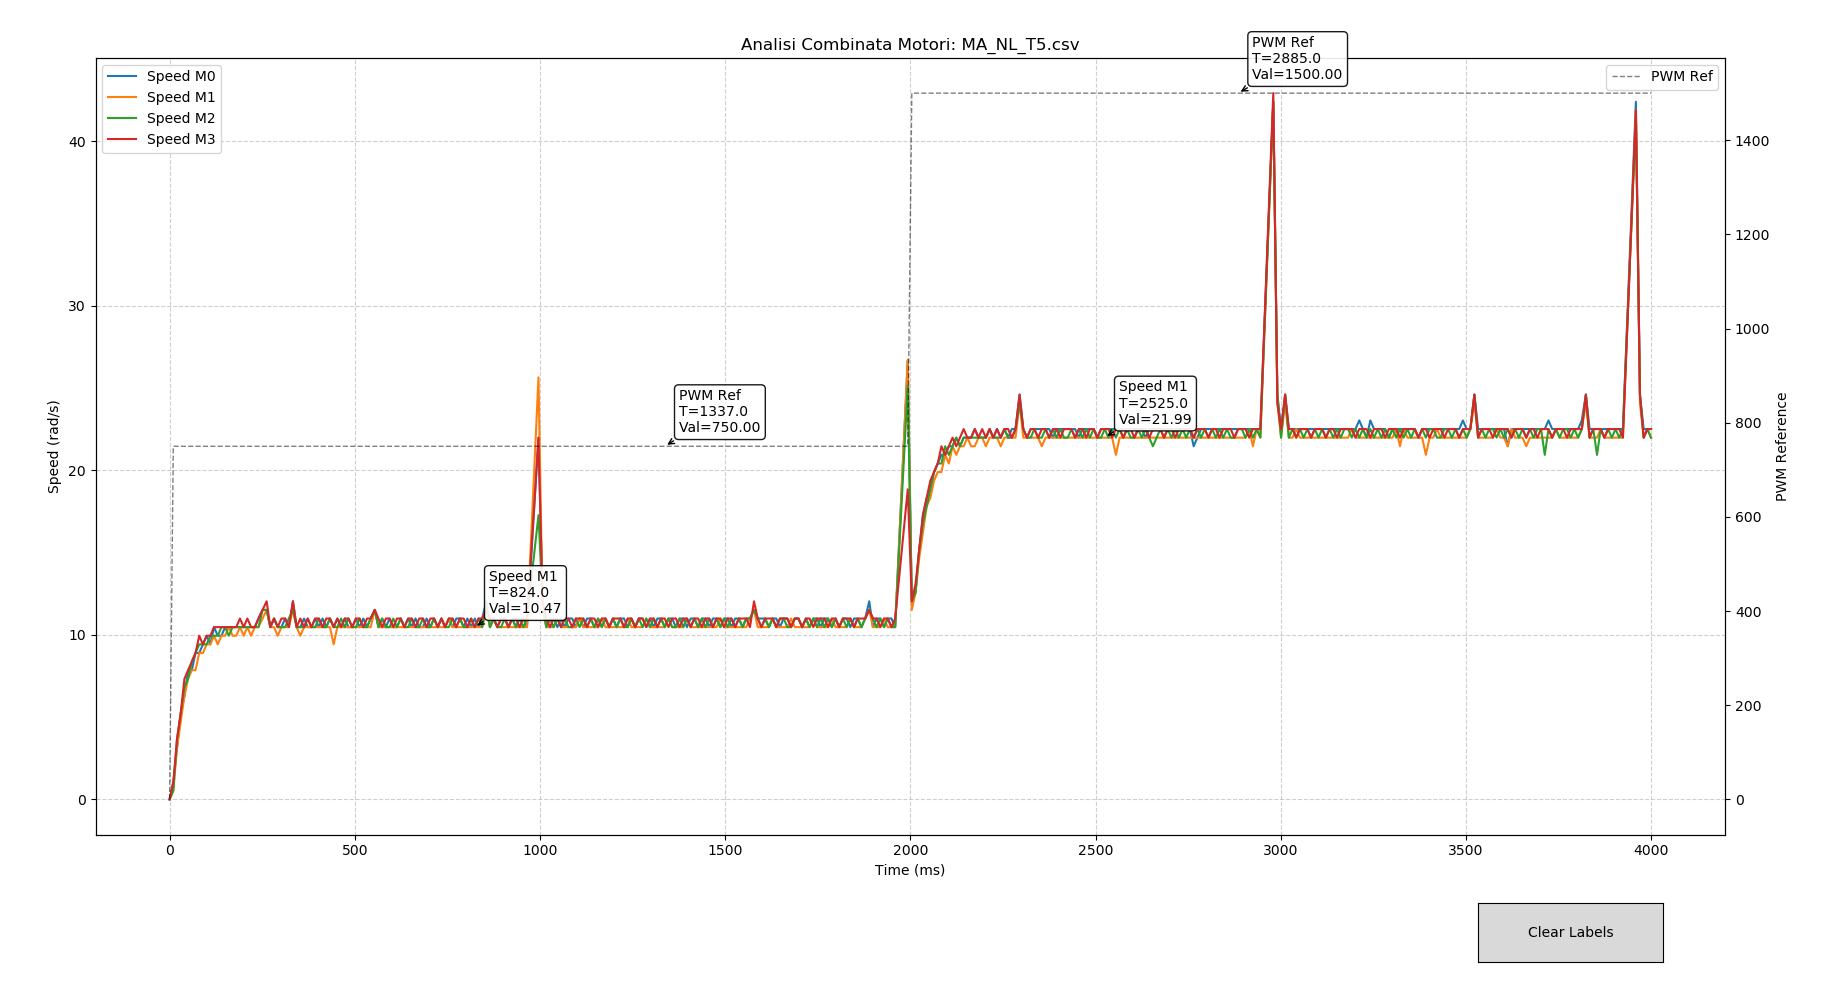
\includegraphics[width=1\textwidth]{IMG/PID/MA_NL_T5_100hz.png}
    \caption{Open-loop test results at 100 Hz showing the initial linear noise increase}
    \label{fig:MA_NL_T5_100hz}
\end{figure}

\begin{vscode}{main.cpp/loop\_tuning}
void loop() {
  ArduinoOTA.handle();
  server.handleClient();  
  handleOfflineTest(); // Controlla pressione tasto

  // Gestione Countdown 5 secondi dopo press BOOT
  if (is_boot_test_pending) {
    if (millis() - boot_test_start_millis > 5000) {
      is_boot_test_pending = false;
      
      // AVVIO TEST E LOG
      logFile = SPIFFS.open("/log.csv", "w");
      if (logFile) {
        tuner.setOutput(&logFile);
        //start(maschera motori attivi, pwm_max, preheat time, step1_time, step2_time)
        tuner.start(0b1111, 1500, 0, 2000, 2000); 
      }
    }
  }

  // Se il tuner è attivo, esegui il suo ciclo di update (non bloccante)
  if (tuner.isRunning()) {
    // Controllo ABORTO: Se premi 'x'
    // (Solo se connesso via seriale)
    if (Serial.available() > 0) {
      char c = Serial.peek(); // Guarda il carattere senza rimuoverlo subito
      if (c == 'x' || c == 'X') {
        Serial.read(); // Rimuovi dal buffer
        tuner.stop();
        return; // Ricomincia il loop
      }
    }
    tuner.update();
  }
  // Chiusura del file log
  else if (logFile) {
    logFile.close();
    tuner.setOutput(&Serial); 
    Serial.println("\n--- LOG SALVATO SU SPIFFS ---");
    Serial.println("Usa il comando 'r' per scaricare i dati.");
  }
  // Altrimenti attendi comandi seriali
  else {
    handleSerialInput();
  }
}
\end{vscode}


\subsection{Closed-Loop}
The transition from open-loop duty cycle commands to a regulated velocity setpoint was achieved through a Proportional-Integral (PI) controller. Since the plant is modeled as a stable first-order system with no zeros, a PI architecture is sufficient to ensure a null steady-state error for step references $R(s) = \frac{1}{s}$.

\subsubsection{Controller Design and Pole-Zero Cancellation}
\begin{figure}[H]
    \centering
    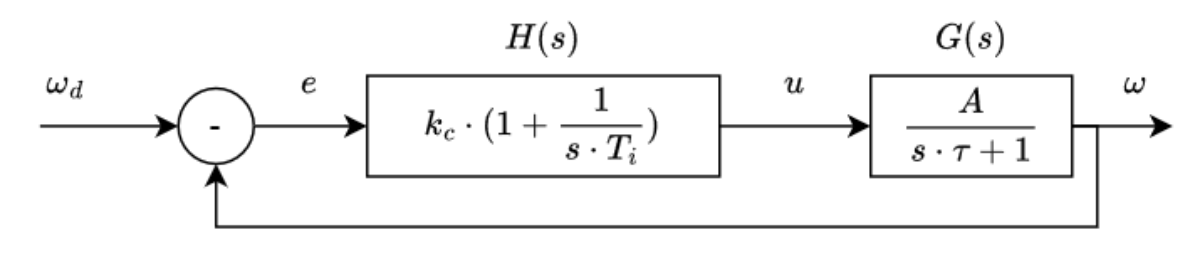
\includegraphics[width=1\textwidth]{IMG/PID/PI_Arch.png}
    \caption{Closed-Loop system - Block diagram}
    \label{fig:PI_Arch}
\end{figure}
Consider the controlling architecture presented in Figure : \ref{}
The controller $H(s)$ is defined by the following transfer function:
\begin{equation}
    H(s) = k_c \left( 1 + \frac{1}{T_i s} \right) = k_c \frac{T_i s + 1}{T_i s}
\end{equation}
where $k_c$ represents the proportional gain and $T_i$ the integral time constant. To simplify the closed-loop dynamics, the design choice $T_i = \tau$ was adopted. This allows the controller's zero to cancel the plant's pole, resulting in the open-loop transfer function:
\begin{equation}
    G(s)H(s) = k_c \frac{A}{\tau s + 1} \cdot \frac{\tau s + 1}{\tau s} = \frac{k_c A}{\tau s}
\end{equation}
The resulting closed-loop transfer function remains a first-order system with unity gain ($A_{cl} = 1$):
\begin{equation}
    T(s) = \frac{G(s)H(s)}{1 + G(s)H(s)} = \frac{1}{\tau_{cl} s + 1}, \quad \text{with } \tau_{cl} = \frac{\tau}{k_c A}
\end{equation}

\subsubsection{Feedforward Compensation and Real-world Constraints}
\begin{figure}[H]
    \centering
    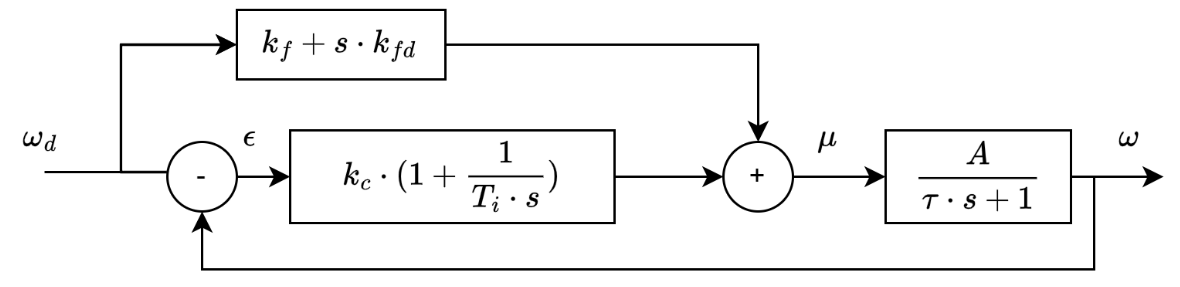
\includegraphics[width=1\textwidth]{IMG/PID/PI_FF_Arch.png}
    \caption{Closed-loop control architecture with feedforward - Block diagram}
    \label{fig:PI_FF_Arch}
\end{figure}
Consider the controlling architecture presented in Figure  \ref{fig:PI_FF_Arch}
To enhance the system's reactivity beyond the feedback loop's limits, a Feedforward (FF) action $F(s)$ was considered. Ideally, the FF controller should invert the plant dynamics ($F(s) = 1/G(s)$) to achieve $F(s)G(s) = 1$. However, a full inversion $\frac{\tau s + 1}{A}$ would be non-proper, requiring a derivative term $k_d$ that is physically unrealizable and highly sensitive to noise. 
Therefore, a simplified feedforward gain was implemented as the inverse of the steady-state gain:
\begin{equation}
    k_f = \frac{1}{A}
\end{equation}
This allows the system to reach the setpoint in finite time by providing the theoretical steady-state voltage required, while the PI controller manages parameter uncertainties and disturbances.

\subsubsection{Experimental Validation and Tuning Strategy}
Initial tuning was performed using a baseline configuration where the desired closed-loop time constant was set to the open-loop value ($\tau_{cl} = \tau$).
\begin{vscode}{robot\_config.h/}
// PI Gains (Derived via IMC Tuning) 
const float kMotCtrlTauCl = kMotModelTau / 1.0f;   
// Desired time constant for the closed-loop (s)
const float kMotCtrlKcKp = kMotModelTau / (kMotCtrlTauCl + kMotModelLag);   
// Tuning: Kc_PI * Kp_plant
const float kMotCtrlKc = (kMotModelTau / kMotCtrlTauCl) / kMotModelKp;  
// PI proportional gain (V / rad.s^(-1))
const float kMotCtrlTi = kMotModelTau;
// PI integration time (s)
const float kMotCtrlKf = 1.0f / kMotModelKp;
// Feed-Forward gain
\end{vscode}

As shown in Fig. \ref{fig:PID_15Rad_200hz_FF}, this configuration led to an overshoot of approximately 20\% and significant jitter at high frequencies (200 Hz). This behavior is consistent with the theoretical risks of aggressive feedforward and quantization errors in discrete-time systems.

To ensure stability without overshoot, a conservative tuning was finalized by doubling the closed-loop time constant ($\tau_{cl} = 2\tau$) and disabling the feedforward action ($k_f = 0$). 
\begin{equation}
    \tau_{cl} = 2 \cdot \tau \implies k_c = \frac{\tau}{2 \tau A} = \frac{1}{2A}
\end{equation}
The results, validated at 50 Hz (Fig. \ref{fig:PID_20Rad_50hz_NoFF}), demonstrate a purely asymptotic response. This configuration successfully balances the convergence speed with the necessity of a high Signal-to-Noise Ratio (SNR) in velocity estimation.
% --- PID Closed Loop Tests ---
\begin{figure}[H]
    \centering
    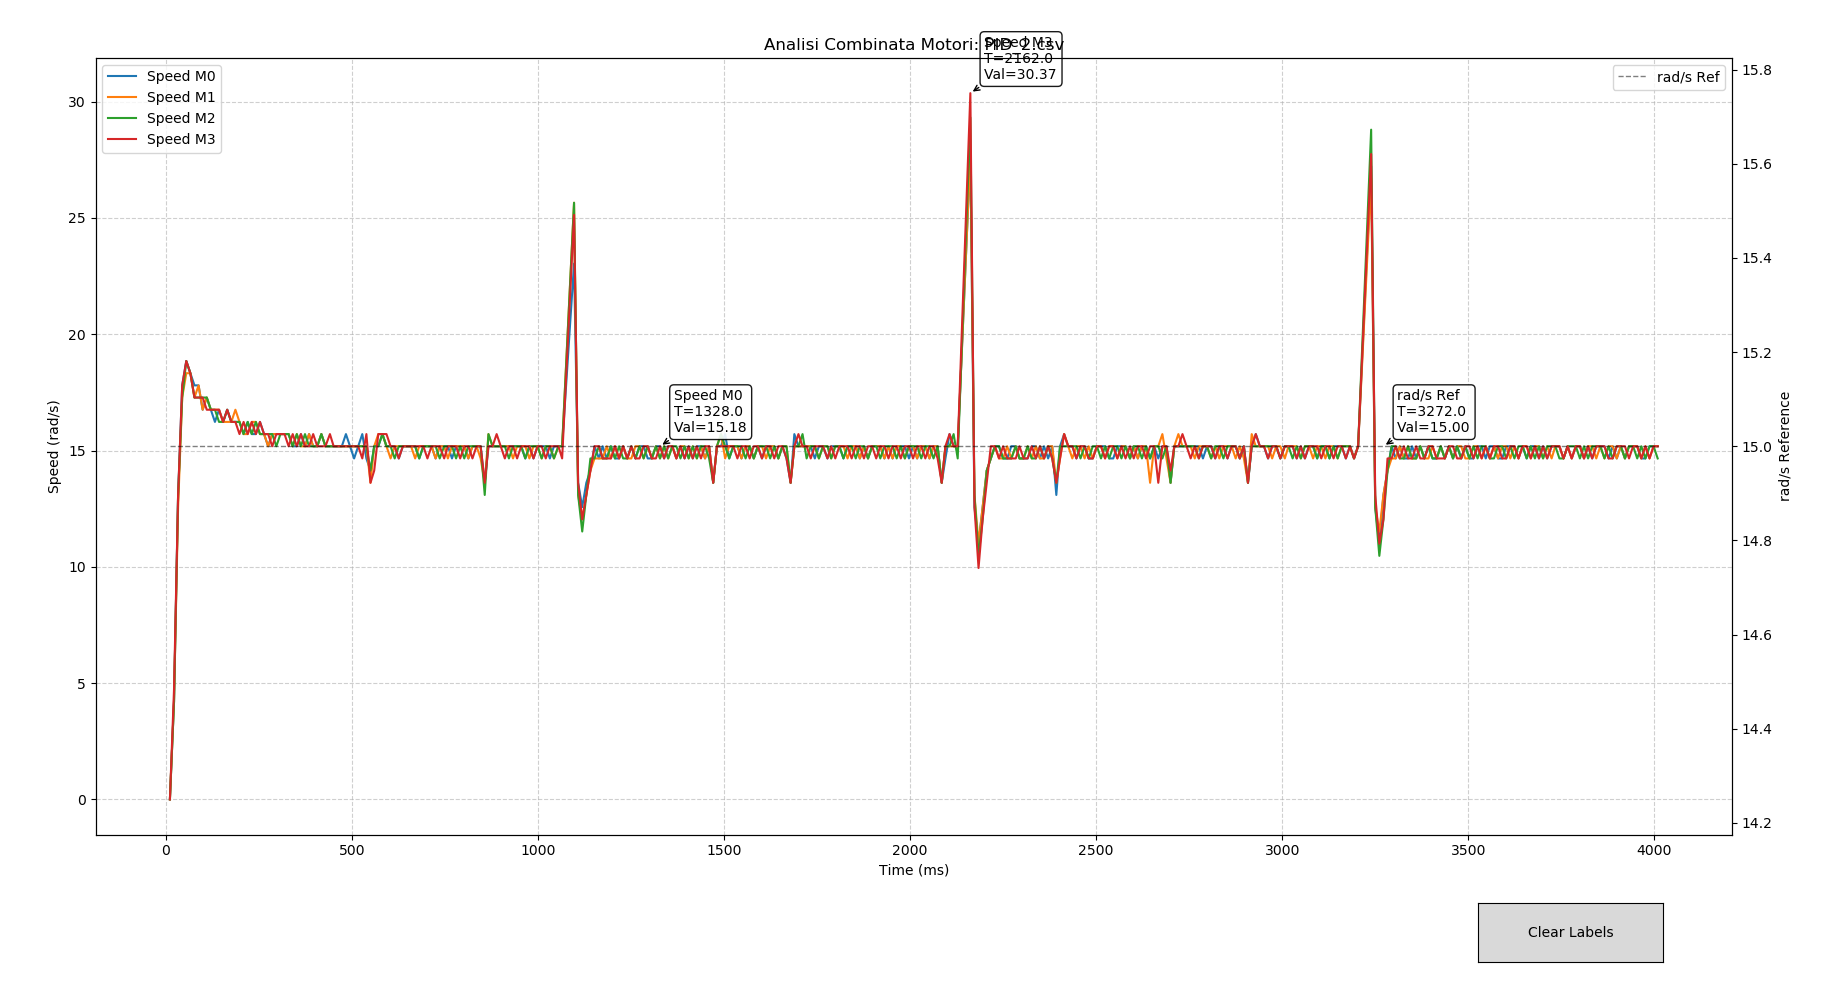
\includegraphics[width=1\textwidth]{IMG/PID/PID_15Rad_200hz_Feedforward_CloseLoop.png}
    \caption{Full closed-loop PID test at 15 rad/s (200 Hz) with Feedforward compensation}
    \label{fig:PID_15Rad_200hz_FF}
\end{figure}

\begin{figure}[H]
    \centering
    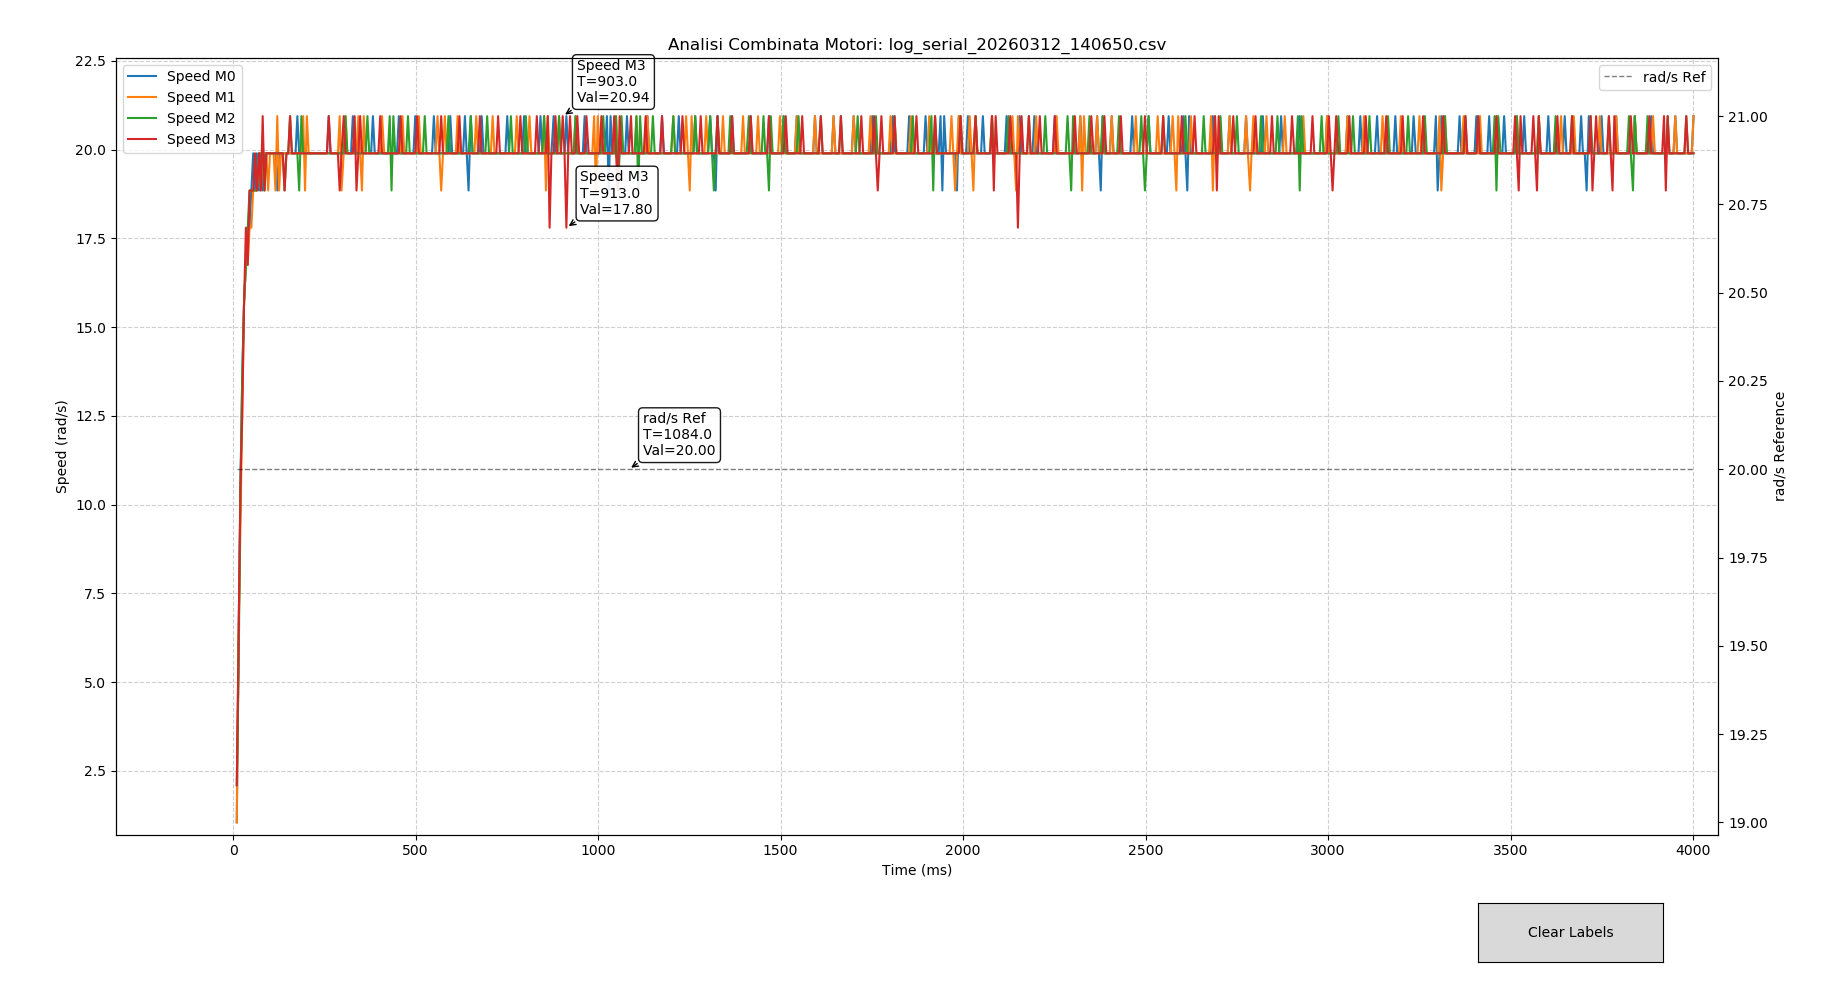
\includegraphics[width=1\textwidth]{IMG/PID/PID_20Rad_100hz_NoFeedforward_CloseLoopHalf.png}
    \caption{PID closed-loop response at 20 rad/s (100 Hz) showing increased measurement jitter}
    \label{fig:PID_20Rad_100hz_NoFF}
\end{figure}

\begin{figure}[H]
    \centering
    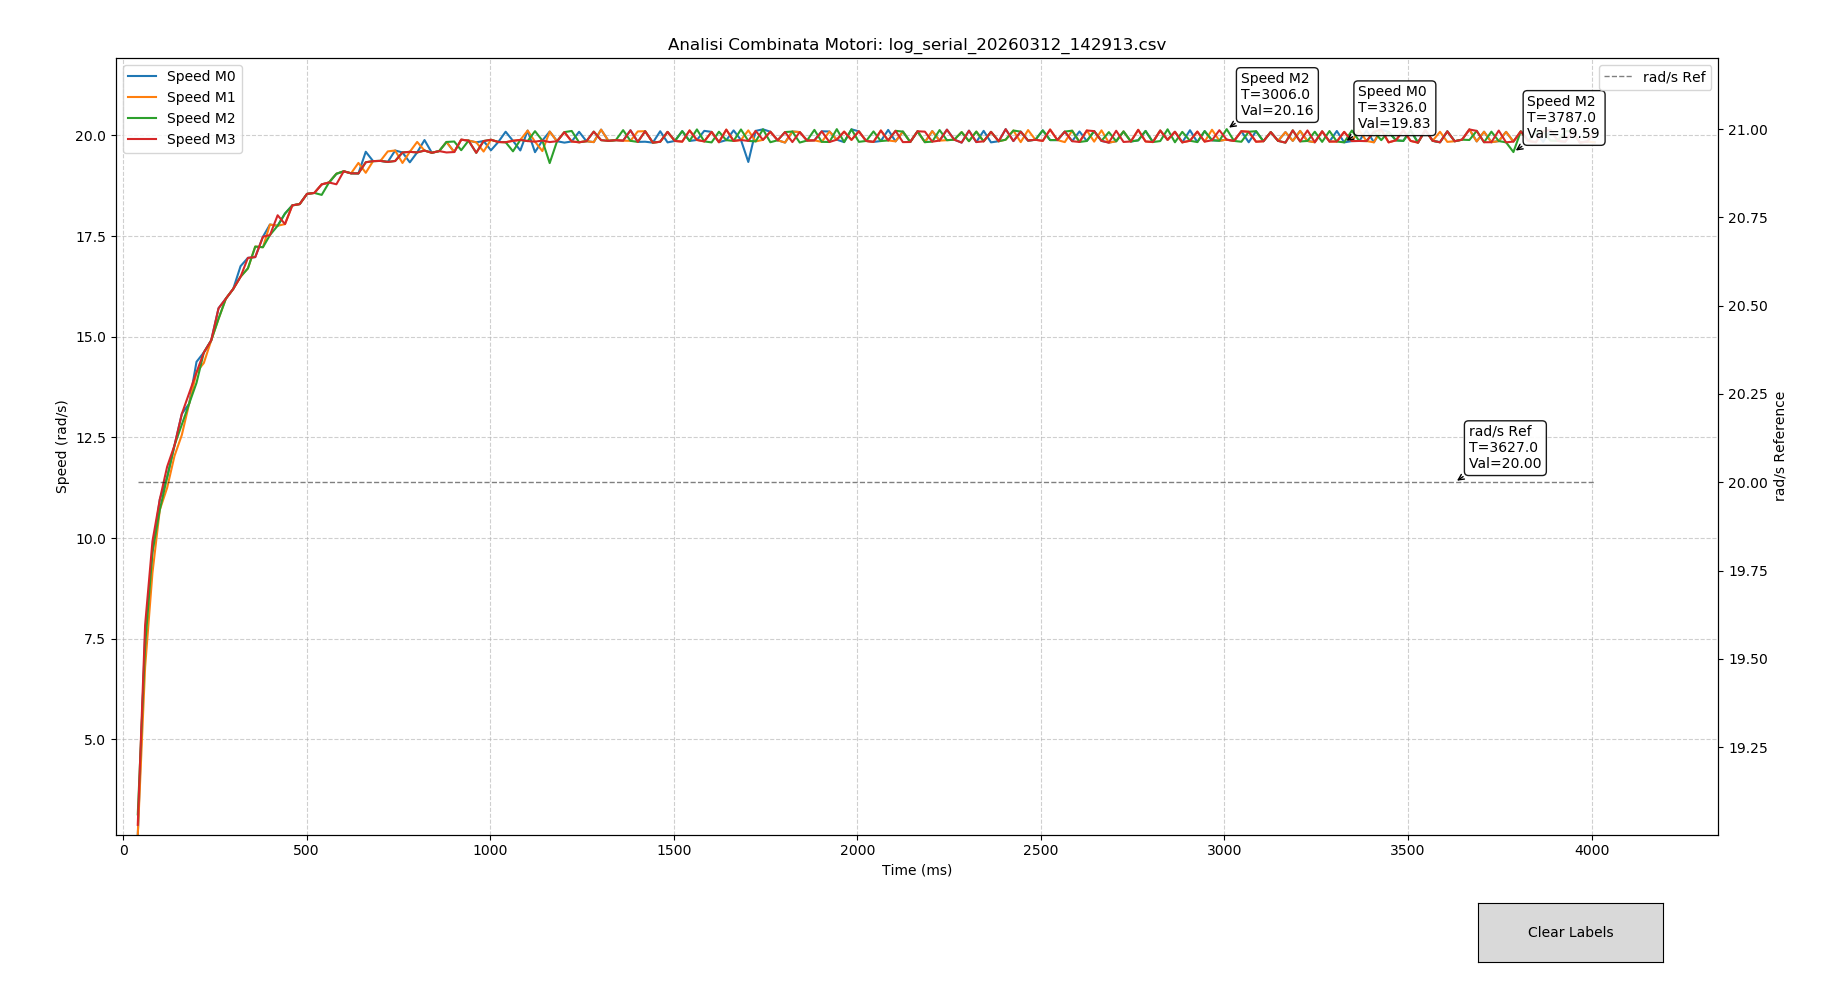
\includegraphics[width=1\textwidth]{IMG/PID/PID_20Rad_50hz_NoFeedforward_CloseLoopHalf.png}
    \caption{PID closed-loop tracking at 20 rad/s (50 Hz) without Feedforward}
    \label{fig:PID_20Rad_50hz_NoFF}
\end{figure}


